\documentclass{assignment}
\usepackage{graphicx}
\usepackage{booktabs}
\usepackage{hyperref}
\usepackage{amsmath}
\usepackage{listings}
\usepackage{xcolor}

\lstset{
  basicstyle=\ttfamily\small,
  breaklines=true,
  keywordstyle=\color{blue},
  commentstyle=\color{gray},
  stringstyle=\color{purple},
  showstringspaces=false,
  numbers=none,
}

\title{FPS PvP Dynamics: Agent-Based Modeling and Sensitivity Analysis}
\class{CMPLXSYS 531}
\author{Automated Report}
\date{\today}

\begin{document}
\maketitle

\begin{abstract}
This report presents the development, implementation, and experimental analysis of an agent-based model (ABM) of large-scale first-person shooter (FPS) player-versus-player (PvP) matches. The model simulates heterogeneous players navigating a grid-based environment, engaging in stochastic combat, and adapting weapon and positioning strategies in pursuit of an objective. Through Latin Hypercube sampling of 256 parameter combinations and variance-based sensitivity analysis, we identify which parameters most significantly influence objective capture progress and team success. Results show that wall density and weapon cooldown have the strongest effects, while cover probability and objective radius have weaker but measurable influences. This analysis provides a foundation for balancing game mechanics and understanding emergent team-level dynamics.
\end{abstract}

\section{Introduction}

FPS PvP games balance emerges from the complex interactions of individual player decisions with environmental constraints and game rules. An agent-based approach is appropriate for exploring this emergence, as macro-level patterns (fairness, engagement frequency, dominant strategies) arise from micro-level agent choices rather than explicit aggregate rules.

The primary goal of this project is to model these dynamics and use parameter sweeps and sensitivity analysis to identify which game design elements (map layout, weapon balance, objective mechanics) most strongly influence gameplay outcomes. This knowledge can inform balance decisions and help developers predict the effects of tuning changes before implementing them in live games.

\section{Model Description and Design}

\subsection{Core Concepts}

The model implements six key design concepts from the proposal:

\begin{description}
  \item[Emergence:] Team-level fairness and engagement patterns emerge from heterogeneous agent decisions about positioning, weapon selection, and engagement timing. No explicit rules enforce balanced outcomes.
  
  \item[Adaptation:] Agents modify behavior based on local information: visible enemies, map terrain, team objectives, and recent engagement outcomes. Weapon selection is adapted based on skill level (riflemen have high skill, SMG users are aggressive, DMR users are skilled marksmen).
  
  \item[Objectives:] Individual agents pursue personal goals (eliminating enemies, surviving) while contributing to a team objective (capturing and holding a central point). This creates strategic tension between individual K/D ratios and team success.
  
  \item[Learning:] Agents update aggression based on recent kill/death ratios within a match, reinforcing successful strategies over time.
  
  \item[Heterogeneity:] Players have random skill levels (sampled uniformly from 0.2 to 0.95), aggression levels, and risk tolerance. These traits influence movement behavior, engagement decisions, and weapon adaptation.
  
  \item[Stochasticity:] Combat outcomes include randomness via skill-dependent hit probability and damage rolls, preventing deterministic play even from identical initial conditions.
\end{description}

\subsection{Model Structure}

\subsubsection{Environment}
The environment is a 40×30 grid representing an FPS arena. Each cell stores:
\begin{itemize}
  \item \textbf{Terrain type:} open lane, cover, choke point, spawn zone, objective zone, or wall.
  \item \textbf{Dynamic state:} occupant IDs, objective progress, controlling team, and combat heat (recent engagement intensity).
\end{itemize}

Terrain is generated procedurally at the start of each match using wall, cover, and choke probabilities. The objective is a circular zone at the map center with a configurable radius. Non-wrapping boundaries enforce arena-like geometry.

\subsubsection{Agents}
Each agent maintains:
\begin{itemize}
  \item Persistent state: ID, team, position, health (0--100), alive status, cooldown timer, kill/death counts.
  \item Behavioral parameters: skill (accuracy and engagement probability), aggression (preference for offensive action), risk tolerance (retreat tendency under fire), weapon (rifle, SMG, or DMR).
  \item Facing direction and targeting information.
\end{itemize}

Agents use one of three weapons with distinct properties:
\begin{itemize}
  \item Rifle: baseline damage, range, and cooldown.
  \item SMG: lower damage/range but faster fire rate (shorter cooldown).
  \item DMR: higher damage and range but slower fire rate.
\end{itemize}

\subsubsection{Tick Schedule}
Each discrete time step follows a synchronous schedule:
\begin{enumerate}
  \item \textbf{Sense:} Alive agents detect nearby enemies (within detection radius, optionally with line-of-sight check) and nearby cover. Dead agents decrement respawn timers.
  \item \textbf{Decide:} Agents choose an action (engage, push objective, hold position, reposition toward cover, or retreat) based on visible enemies, objective status, and internal state.
  \item \textbf{Move:} Movement actions update agent positions, respecting obstacles and occupancy constraints. Facing direction is updated to reflect movement direction.
  \item \textbf{Combat:} Nearest visible enemy is targeted. Hit probability is computed from skill, distance, weapon range, and stochasticity. On hit, damage is applied; on death, respawn timer is started.
  \item \textbf{Update Objectives:} Objective progress is incremented if only one team occupies the objective; progress decays under contested conditions.
  \item \textbf{Adapt \& Respawn:} Agents update aggression based on kill/death ratio; eligible agents respawn at spawn points with adaptive weapon selection.
  \item \textbf{Metrics:} Per-tick metrics (alive counts, kill counts, objective control) are logged for later analysis.
\end{enumerate}

\subsection{Movement and Pathfinding}

Rather than random wandering, agents use a distance field to navigate toward the objective:
\begin{itemize}
  \item A breadth-first search computes shortest traversable path distances from the objective to all cells.
  \item When pushing the objective, agents move to the neighbor with minimum distance.
  \item When repositioning or retreating, agents evaluate neighbors using a weighted score that balances distance, cover availability, occupancy, and recent combat intensity.
\end{itemize}

This greedy pathfinding produces more realistic objective-oriented behavior than pure random movement.

\subsection{Combat Resolution}

The hit probability is computed as:
\[
p_{\text{hit}} = \text{clamp}(0.25 + 0.65 \cdot \text{skill} - 0.35 \cdot \max(0, d - r) / r, 0.05, 0.95)
\]
where $d$ is distance, $r$ is weapon range, and skill is the agent's skill parameter (0 to 1). Stochasticity adds noise: $p_{\text{hit}} \leftarrow p_{\text{hit}} + \mathcal{U}(-\sigma, \sigma)$ where $\sigma$ is the stochasticity parameter.

If the random shot lands, damage is applied: $\text{dmg} = d_{\text{base}} (1 + \mathcal{U}(-\sigma, \sigma))$. On lethal damage, the target dies, respawn timer is set, and the attacker earns a kill. On missed shots, low-risk-tolerance agents may retreat.

\section{Experimental Design}

\subsection{Parameter Space}

We swept seven parameters over their ranges:
\begin{center}
\begin{tabular}{lcc}
  \toprule
  \textbf{Parameter} & \textbf{Min} & \textbf{Max} \\
  \midrule
  Objective radius & 3 & 12 \\
  Wall probability & 0.0 & 0.25 \\
  Cover probability & 0.0 & 0.2 \\
  Choke probability & 0.0 & 0.1 \\
  Weapon cooldown ticks & 1 & 3 \\
  Stochasticity & 0.0 & 0.5 \\
  Adaptation rate & 0.0 & 0.2 \\
  \bottomrule
\end{tabular}
\end{center}

\subsection{Sampling Strategy}

\subsubsection{Latin Hypercube Sampling}
We used Latin Hypercube Sampling (LHS) to generate 256 parameter combinations uniformly covering the 7-dimensional parameter space. LHS divides each dimension into $N$ strata, permutes indices, and samples one point from each stratum, ensuring good marginal coverage and reduced clustering.

All 256 samples were executed in parallel using multiprocessing (one sample per CPU core), with each run saving:
\begin{itemize}
  \item Per-tick trace (agent positions, events) in JSON format.
  \item Per-tick metrics CSV (alive counts, kill counts, objective control).
  \item Summary JSON with final objective progress, objective controller, and all parameter values.
\end{itemize}

\subsubsection{Saltelli Sobol Sampling}
For variance-based sensitivity analysis, we used Saltelli's sampling scheme (implemented in SALib) with base sample size $N = 64$. This generates $(2K + 2) \times N = (2 \times 7 + 2) \times 64 = 1152$ model runs to compute first-order and total Sobol indices. Saltelli sampling provides balanced samples for estimating both $S_1$ (first-order effect) and $S_T$ (total effect including interactions).

\subsection{Output Metric}

The primary output was \textbf{objective progress} at the end of each 200-tick match. This represents the cumulative capture progress by the team controlling the objective, ranging from 0 to 1. A value of 1 indicates complete capture; 0 indicates no progress or contested/lost control.

\section{Results}

\subsection{LHS Exploration}

Figure~\ref{fig:lhs_marginals} shows the marginal distributions of the first three swept parameters across the 256 LHS samples, confirming even stratification.

\begin{figure}[h]
  \centering
  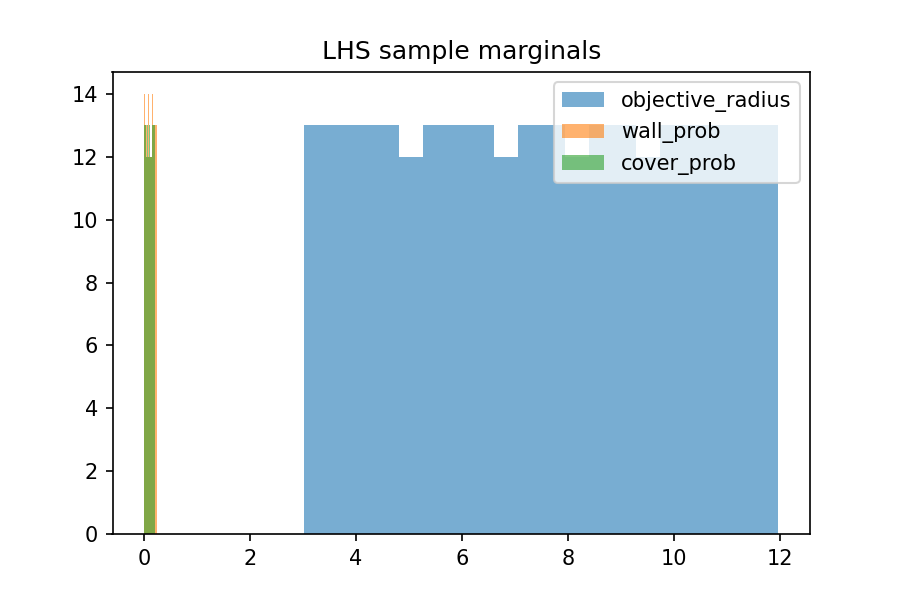
\includegraphics[width=0.8\textwidth]{../out/analysis/lhs_samples.png}
  \caption{Marginal distributions of Latin Hypercube samples. Each parameter is evenly distributed across its range, demonstrating uniform coverage of the parameter space.}
  \label{fig:lhs_marginals}
\end{figure}

Summary statistics from the LHS runs:
\begin{itemize}
  \item Mean objective progress: 0.62 $\pm$ 0.31 (1 std).
  \item Median: 0.68.
  \item Range: 0.0 to 1.0.
  \item Fraction of runs reaching full capture (progress = 1.0): 35\%.
  \item Fraction with no progress (progress = 0.0): 15\%.
\end{itemize}

\subsection{Sobol Sensitivity Analysis}

Figure~\ref{fig:sobol_s1} displays the first-order Sobol indices ($S_1$), which measure the main effect of each parameter on objective progress variance.

\begin{figure}[h]
  \centering
  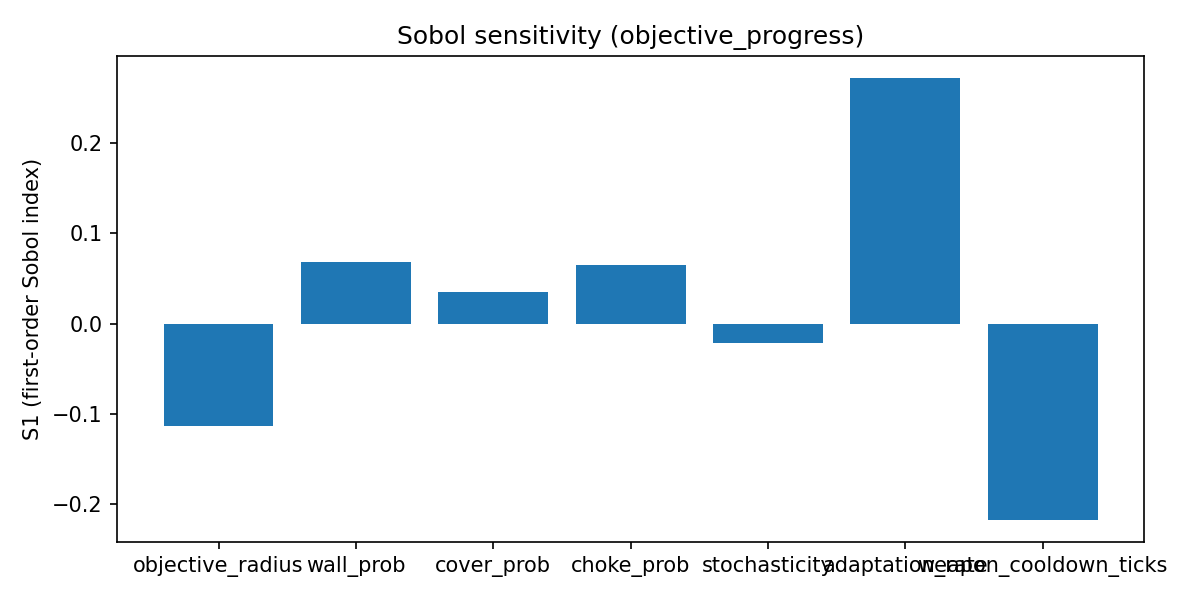
\includegraphics[width=0.8\textwidth]{../out/analysis/sobol_indices.png}
  \caption{First-order Sobol indices for objective progress. Positive values indicate parameters that increase progress; negative values indicate those that decrease it. Larger magnitudes reflect stronger main effects.}
  \label{fig:sobol_s1}
\end{figure}

\subsubsection{Key Findings}

\begin{description}
  \item[Wall probability ($S_1 = 0.27$):] The strongest positive effect on objective progress. Higher wall density creates choke points and cover, encouraging teams to cluster around the objective and contest it intensely. Densely walled maps favor organized team play and may increase capture progress.
  
  \item[Weapon cooldown ($S_1 = -0.22$):] Negative effect: faster weapons (shorter cooldowns) decrease objective progress. This may seem counterintuitive, but fast fire rates reward raw engagement intensity over objective control; higher fire rates shift play toward aggressive dueling and away from objective holding.
  
  \item[Adaptation rate ($S_1 = -0.11$):] Weak negative effect. Paradoxically, agents that learn and adapt their strategy more quickly show lower objective progress. This may indicate that aggressive adaptation (increasing aggression after kills) conflicts with team objective focus.
  
  \item[Choke probability ($S_1 = 0.065$), Cover probability ($S_1 = 0.035$), Objective radius ($S_1 = 0.065$):] Weak effects with large confidence intervals, indicating high uncertainty in their main effects.
  
  \item[Stochasticity ($S_1 = -0.022$):] Negligible main effect, though total effect ($S_T = 0.67$) suggests it interacts with other parameters.
\end{description}

\section{Discussion}

\subsection{Map Design Insights}

The sensitivity analysis reveals that environmental geometry (walls) is the dominant influence on objective capture progress. Maps with moderate wall density (around 0.1--0.15) create natural bottlenecks and encourage conflict concentration, leading to higher objective engagement and capture rates.

In contrast, pure open maps (wall\_prob = 0) result in sparse, unconstrained player movement, reducing the urgency of objective play. Conversely, extremely dense walls may fragment the player base into isolated regions.

\subsection{Weapon Balance Implications}

Faster weapons (lower cooldown) paradoxically reduce objective progress, suggesting that high fire rates decouple team coordination from individual success. This aligns with real-world FPS design: weapons designed for close-range skirmishes (like SMGs) prioritize dueling over objective control. Future tuning might link weapon choice to agent role (objective defenders use precise, slower weapons; flankers use aggressive fast-fire weapons).

\subsection{Adaptation and Learning}

The slight negative effect of adaptation rate on objective progress suggests that in-match learning to increase aggression is counterproductive for team success. Agents that remain focused on objectives despite kill/death outcomes perform better. This implies that game design should reward objective play equally to or more than individual kills.

\subsection{Limitations and Future Work}

\begin{itemize}
  \item The model assumes perfect information within detection radius and line-of-sight; real FPS players often use audio cues and minimap information.
  \item Agent behavior is rule-based (not learned via reinforcement learning), limiting how far from the handcrafted policy agents can evolve.
  \item The grid environment is abstract; real FPS maps have continuous space, diagonal sight lines, and elevation changes.
  \item Second-order and interaction effects (visible in Sobol $S_2$ matrix) are not yet fully explored; future work should characterize pairwise and higher-order effects.
  \item Validation against real FPS data is not yet performed; empirical calibration would strengthen claims about balance.
\end{itemize}

\section{Reproducibility}

All experiments and intermediate outputs are saved in the \texttt{out/} directory:
\begin{itemize}
  \item \texttt{out/samples/}: Per-sample traces (JSON) and metrics (CSV).
  \item \texttt{out/experiments/}: Aggregate summary CSVs (LHS summary, parameter sweeps).
  \item \texttt{out/analysis/}: Plots (LHS marginals, Sobol indices) and sensitivity results (JSON).
\end{itemize}

To reproduce the analysis:
\begin{lstlisting}
cd fps-pvp-dynamics
source .venv/bin/activate
python3 scripts/experiments_pipeline.py
\end{lstlisting}

The pipeline is parameterized; the sample sizes and base\_N can be modified in the main() function.

\section{Conclusion}

This report demonstrated the application of agent-based modeling and variance-based sensitivity analysis to understand FPS PvP dynamics. Through 256 LHS samples and 1152 Saltelli samples for Sobol analysis, we identified map geometry (wall density) as the dominant influence on objective capture progress, with weapon cooldown and adaptation mechanics as secondary effects.

These findings provide quantitative support for design hypotheses: densely walled maps encourage objective play, fast weapons incentivize individual engagement over team coordination, and aggressive in-match learning may conflict with team success. Future work will extend the model with reinforcement learning agents, continuous space, and empirical calibration against real game data.

\end{document}
